This chapter continues looking at the case where the MDP models are
large state space. In the previous chapter we looked at
approximating the value function. In this chapter we will consider
learning directly a policy and optimizing it.

The main advantages and disadvantages of policy optimization (rather
than value function approximation) are the following:
\begin{enumerate}
\item
Continuous action space. In such a case the policy optimization
method is the most natural and the one which is used in practice
(for applications such as robotics).
\item
Convergence: While the policy optimization would normally converge,
it will most likely converge to a local optimum.
\item
High dimensional spaces: It can be fairly effective in selecting the
actions (in contrast to learning accurate values).
\item
Evaluation time would typically be longer (compared to value
function approaches).
\item
Stochastic Policy: allows naturally to have a stochastic policy.
\end{enumerate}

\section{Stochastic policies}

We have seen that the optimal policy in an MDP is deterministic, so
what benefit can be in considering a stochastic policy?

The main benefit is in situations where there is a
miss-specification of the model. The main issue is that the state
encoding might create a system which is not Markovian anymore, by
coalescing certain states which have identical encoding. We will
give two example of this phenomena.

\paragraph{Aliased Grid-world}\ \\
Consider the example in Figure~\ref{fig:L9-grid-world}. The green
state is the good goal and the red ones are the bad. The encoding of
each state is the location of the walls. In each state we need to
choose a direction. The problem is that we have two states which are
indistinguishable (marked by question mark).

It is not hard to see that any deterministic policy would fail from
some start state (either the left or the right one). Alternatively,
we can use a randomized policy in those states,with probability half
go right and probability half go left. For such a policy we have a
rather short time to reach the green goal state (and avoid the red
states).

The issue here was that two different states had the same encoding,
and thus violated the Markovian assumption. This can occur when we
encode the state with a small set of features, and some (hopefully,
similar) states coallesce to a single representation.

\begin{figure}
  % Requires \usepackage{graphicx}
  \begin{centering}
  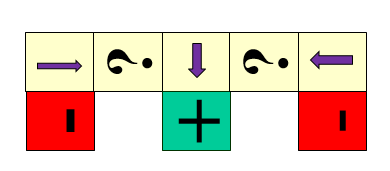
\includegraphics[width=0.5\textwidth]{figures/L9-grid-world.png}\\
  \caption{Grid-world example }\label{fig:L9-grid-world}
  \end{centering}
\end{figure}

\paragraph{Zero-sum games}\ \\
The MDP model was not designed for interactive zero-sum games,
however, in many of the applications we saw, we train a policy to
play a board game (such as backgammon). Any board game is an
instance of a zero-sum game, since if one player wins the other
loses. In alternating-moves games, the optimal policy would still be
deterministic, but this is not the case in simultaneous-move games.

%The main issue with a more general game, is the the optimal policy
%might be stochastic.

Consider a penny-matching game, in which each player simultaneously
select a bit $\{0,1\}$. If the two selected bits are identical the
first player wins and if they differ the second player wins. The
best policy for each player is stochastic (selecting each bit with
probability half).

An important observation is that if one of the players plays
deterministically (or almost deterministically), then the other
player can win (or almost always win) by selecting
(deterministically) the appropriate action. For this reason, even
an $\varepsilon$-greedy would have a poor performance.

Here we violated the assumption that the rewards depend only on the
state. In this example they depend indirectly on the policy selected by the opponent player.

\section{Policy optimization}

We will assume that each state $\state$ has an encoding
$\phi(\state)\in \mathbb{R}^{d_1}$. The policy will have a
parametrization $\theta\in \mathbb{R}^{d_2}$. The policy will be
based on the two encodings, and we have
$\policy(\action|\state,\theta)$, which is the probability of
selecting action $\action$ when observing state $\state$ (or,
equivalently, $\phi(\state)$), and having a policy parametrization
$\theta$.

The optimization problem would be:
\[
\theta^* = \arg\max_\theta J(\theta)
\]
where $J(\theta) \triangleq \Value^\policy(\state_0)$ is the
expected return of the policy $\policy(\cdot|\cdot,\theta)$ from the
initial state $\state_0$.
%
This maximization problem can be solved in multiple ways. We will
mainly explore gradient based methods.

We start by giving a few examples on how to parameterize the policy.
The first is a {\em log linear policy}. We will assume an encoding
of the state and action pairs, i.e., $\phi(\state,\action)$. Given the parameter $\theta$, The linear part will compute $\mu(\state,\action)=\phi(\state,\action)^\top \theta$. Given the values of $\mu(\state,\action)$ for each $\action\in \Actions$, the policy select action $\action$ with probability proportional to
$e^{\mu(\state,\action)}$. Namely,
\[
\policy(\action|\state,\theta)=
\frac{e^{\mu(\state,\action)}}{\sum_{b\in
\Actions}e^{\mu(\state,b)}}
\]
Note that this is essentially a soft-max selection over $\mu(\state,\action)$.

The second example is a {\em Gaussian policy}, where the action
space is a real number, i.e., $A=\mathbb{R}$. The encoding is of states, i.e., $\phi(\state)$, and the actions are any real number. Given a state $\state$
we compute $\mu(\state)=\phi(\state)^\top\theta$. We select an
action $\action$ from the normal distribution with mean
$\mu(\state)$ and variance $\sigma^2$, i.e.,
$N(\mu(\state),\sigma^2)$. (The Gaussian policy has an additional
parameter $\sigma$.)

We would like to use the policy gradient to optimize the expected
return  $J(\theta)$ of the policy $\policy(\cdot|\cdot,\theta)$. We
will compute the gradient of $J(\theta)$, i.e., $\nabla_\theta
J(\theta)$. The update of the policy parameter $\theta$ is
\[
\theta_{\ttime+1}=\theta_\ttime + \alpha \nabla_{\theta_\ttime}
J(\theta_\ttime)
\]
where $\alpha$ is a learning rate.

One challenge we will have to address is to relate the global gradient, $\nabla_\theta J(\theta)$, to the local gradients, $\nabla \policy(\action|\state,\theta)$.

\subsection{Finite differences methods}

This methods can be used even when we do not have a representation
of the gradient of the policy or even the policy itself. This may
arise many times when we have, for example, access to an
off-the-shelf robot for which the software is encoded already in the
robot. In such cases we can estimate the gradient by introducing
perturbations in the parameters.

The simplest case is component-wise gradient estimates, which is also named \emph{coordinate ascent} . Let $e_i$ be
a unit vector, i.e., has in the $i$-th entry a value $1$ and a value
$0$ in all the other entries. The perturbation that we will add is
$\delta e_i$ for some $\delta >0$. We will use the following
approximation:
\[
\frac{\partial}{\partial \theta_i}J(\theta)\approx
\frac{\hat{J}(\theta+\delta e_i)-\hat{J}(\theta)}{\delta}
\]
where $\hat{J}(\theta)$ is unbiased estimator of $J(\theta)$. A more
symmetric approximation is sometimes better,
\[
\frac{\partial}{\partial \theta_i}J(\theta)\approx
\frac{\hat{J}(\theta+\delta e_i)-\hat{J}(\theta-\delta e_i
)}{2\delta}
\]

The problem is that we need to average many samples of
$\hat{J}(\theta\pm\delta e_i)$ to overcome the noise. Another
weakness is that we need to do the computation per dimension. In
addition, the selection of $\delta$ is also critical. A small
$\delta$ might have a large noise rate that we need to overcome (by
using many samples). A large $\delta$ run the risk of facing the
non-linearity of $J$.

Rather then performing separately the computation and optimization per dimension, we can perform a more global approach and use a least squares estimation of the gradient.
Consider a random vector $u_i$, then we have
\[
J(\theta+\delta u_i)\approx J(\theta)+\delta u_i^\top \nabla
J(\theta) \;.
\]
We can define the following least square problem,
\[
G= \arg\min_x \sum_i (J(\theta+\delta u_i)- J(\theta)-\delta
u_i^\top x)^2,
\]
where $G$ is our estimate for $\nabla J(\theta)$.

We can reformulate the problem in matrix notation and define $\Delta
J^{(i)}=J(\theta+\delta u_i)- J(\theta)$ and $\Delta J= [\cdots ,
\Delta J^{(i)}, \cdots]^\top$. We define $\Delta \theta^{(i)}=\delta
u_i$, and the matrix $[\Delta\Theta]=[\cdots
\Delta\theta^{(i)},\cdots]^\top$, where the $i$-th row is
$\Delta\theta^{(i)}$.

We would like to solve for the gradient, i.e,
\[
\Delta J\approx [\Delta \Theta]x\;.
\]
This is a standard least square problem and the solution is
\[
G=([\Delta \Theta]^\top [\Delta \Theta])^{-1} [\Delta\Theta]^\top
\Delta J\;.
\]

One issue that we neglected is that we actually do not a have the
value of $J(\theta)$. The solution is to solve also for the value of
$J(\theta)$.
%
We can define a matrix $M=[1, [\Delta\Theta]]$, i.e., adding a column of ones, a vector of unknowns $x=[J(\theta), \nabla J(\theta)]$, and have the target be $z=[\cdots, J(\theta+\delta u_i),\cdots]$. We can now solve for $z\approx Mx$, and this will recover an estimate also for $J(\theta)$.


\section{Policy Gradient Theorem}

The policy gradient theorem will relate the gradient of the expected
return $\nabla J(\theta)$ and the gradients of the policy $\nabla
\policy(\action|\state,\theta)$. We will mainly try to make sure
that we are able to use it to get estimates, and the quantities
would be indeed observable by the learner.

We will state the policy gradient theorem for the finite-horizon
return, but it also holds for the discounted return and average
reward return. Recall that the finite-horizon return is
$\sum_{\ttime=1}^\tHorizon \reward_\ttime$ and
$\Value^\policy(\state)=E[\sum_{\ttime=1}^\tHorizon
\reward_\ttime|\state_1=\state]$.

\begin{theorem}[Policy Gradient Theorem]
\label{thm:policy-gradient} For any policy
$\policy(\cdot|\cdot;\theta)$, we have
\[
\nabla J(\theta)= \sum_{s\in S} \mu(\state) \sum_{\action\in
\Actions} Q^\policy (\state,\action)\nabla_\theta
\policy(\action|\state;\theta)
\]
where $\mu(\state)=\sum_{\ttime=1}^\tHorizon\Pr[\state_\ttime=\state|\state_1,\theta]$.
\end{theorem}

\begin{proof}
For each state $\state$ we have
\begin{align*}
\nabla \Value^\policy(\state) &= \nabla \sum_\action \policy(\action|\state) Q^\policy(\state,\action)\\
&=\sum_\action  Q^\policy(\state,\action) \nabla \policy(\action|\state) + \policy(\action|\state) \nabla Q^\policy(\state,\action)\\
&=\sum_\action  Q^\policy(\state,\action) \nabla \policy(\action|\state) + \policy(\action|\state) \sum_{\state_1} p(\state_1|\state,\action) \nabla \Value^\policy(\state_1)\\
&= \sum_\action  Q^\policy(\state,\action) \nabla
\policy(\action|\state) + \sum_{\state_1} p(\state_1|\state)
\nabla \Value^\policy(\state_1)\\
&= \sum_\action  Q^\policy(\state,\action) \nabla
\policy(\action|\state) + \sum_{\state_1} p(\state_1|\state)
\sum_\action Q^\policy(\state_1,\action) \nabla
\policy(\action|\state_1) + \sum_{\state_2}
p(\state_2|\state_1)p(\state_1|\state)
\nabla \Value^\policy(\state_2)\\
& = \sum_{x\in
S}\sum_{\ttime=1}^\tHorizon\Pr[\state_\ttime=x|\state_1=\state,\policy]\sum_\action
Q^\policy (x,\action)\nabla\policy(\action|x)
\end{align*}
where the first identity follows since by averaging $Q^\policy(\state,\action)$ over the actions $\action$, with the
probabilities induce by $\policy(\action|\state)$, we have both correct expectation of the immediate reward and the next state is distributed correctly. The second equality follows from the gradient of a multiplication, i.e., $\nabla AB=A\nabla B+B\nabla A$. The third follows since 
$\nabla Q^\policy(\state,\action)= \nabla
[\reward(\state,\action)+
\sum_{\state'}p(\state'|\state,\action)\Value^\policy(\state'|\state,\action)]$.
%
The next two identities role the policy one step in to the future.
%
The last identity follows from unrolling $\state_1$ to $\state_2$ etc., and then reorganizing the terms.

Using this we have
\begin{align*}
\nabla J(\theta) &= \nabla \Value^\policy (\state_0)\\
&= \sum_\state \left(\sum_{\ttime=1}^\tHorizon\Pr[\state_\ttime=\state|\state_0,\policy] \right) \sum_\action Q^\policy (\state,\action) \nabla\policy(\action|\state) \\
&= \sum_\state \mu(\state) \sum_\action Q^\policy (\state,\action) \nabla\policy(\action|\state;\theta) \\
%&= \left(\sum_s \eta(\state)\right)\sum_s \frac{\eta(\state)}{\sum_x \eta(x)}  \sum_\action\nabla\policy(\action|\state) Q^\policy (\state,\action) \\
%&= \tHorizon  \sum_s \mu(\state) \sum_\action Q^\policy (\state,\action) \nabla\policy(\action|\state)
\end{align*}
\end{proof}

\begin{example}
Consider an MDP with a single state $\state$ (which is also called
Multi-Arm Bandit, and is discussed in Chapter \ref{chapter:MAB}).
Assume we have only two actions, action $\action_1$ has expected
reward $\reward_1$ and action $\action_2$ has expected reward
$\reward_2$.

The policy $\policy$ is define with a parameter
$\theta=(\theta_1,\theta_2)$, where $\theta_i\in \reals$. Given
$\theta$ the probability of action $\action_i$ is
$p_i=e^{\theta_i}/(e^{\theta_1}+e^{\theta_2})$. We will also select
a horizon of length one, i..e, $\tHorizon=1$. This implies that
$Q^\policy(\state,\action_i)=\reward_i$.

In this simple case we can compute directly $J(\theta)$ and $\nabla
J(\theta)$. The expected return is simply,
\[
J(\theta)=p_1 \reward_1 + p_2 \reward_2 =
\frac{e^{\theta_1}}{e^{\theta_1}+e^{\theta_2}} \reward_1 +
\frac{e^{\theta_2}}{e^{\theta_1}+e^{\theta_2}} \reward_2
\]
Note that $\frac{\partial}{\partial \theta_1} p_1=
p_1-p_1^2=p_1(1-p_1) $ and $\frac{\partial }{\partial \theta_2} p_1=
- p_1 p_2= -p_1(1-p_1)$. The gradient is
\[
\nabla J(\theta)= \reward_1 \begin{pmatrix} p_1(1-p_1)\\
-p_1(1-p_1)\end{pmatrix} + \reward_2 \begin{pmatrix} -p_1(1-p_1)\\
p_1(1-p_1)\end{pmatrix} = (\reward_1-\reward_2) p_1(1-p_1) \begin{pmatrix}+1\\
-1\end{pmatrix}
\]
Updating in the direction of the gradient, in the case that
$\reward_1>\reward_2$, would increase $\theta_1$ and decrease
$\theta_2$, and eventually $p_1$ will converge to $1$.

To apply the Policy gradient theorem we need to compute the
gradient,
\[
\nabla_\theta \policy(\action_1|\state;\theta) = \nabla \begin{pmatrix} p_1\\
1-p_1\end{pmatrix}=  \begin{pmatrix} p_1(1-p_1)\\
-p_1(1-p_1)\end{pmatrix}
\]
and the policy gradient theorem gives us the same expression,
\[
\nabla J(\theta) = \reward_1 \nabla
\policy(\action_1;\theta)+\reward_2 \nabla
\policy(\action_2;\theta)=\reward_1 \begin{pmatrix} p_1(1-p_1)\\
-p_1(1-p_1)\end{pmatrix} + \reward_2 \begin{pmatrix} -p_1(1-p_1)\\
p_1(1-p_1)\end{pmatrix}
\]
where we used the fact that there is only a single state $\state$,
and that $Q^\policy(\state,\action_i)=\reward_i$.
\end{example}

The Policy Gradient Theorem gives us a way to compute the gradient.
We can sample states from the distribution $\mu(\state)$ using the
policy $\policy$. We still need to resolve the sampling of the
action. We are going to observe the outcome of only one action in
state $\state$, and the theorem requires summing over all of them!
In the following we will slightly modify the theorem so that we will
be able to use only the action $\action$ selected by the policy
$\policy$, rather than summing over all actions.

Consider the following simple identity,
\[
\nabla f(x)=f(x)\frac{\nabla f(x)}{f(x)}=f(x)\nabla \log f(x)
\]
This implies that we can restate the Policy Gradient Theorem as the
following corollary,
\begin{corollary}[Policy Gradient Corollary]
\label{thm:policy-gradient} For any policy
$\policy(\cdot|\cdot;\theta)$, we have
\[
\nabla J(\theta)= \sum_{s\in S} \mu(\state) \sum_{\action\in
\Actions} \policy(\action|\state;\theta) Q^\policy
(\state,\action)\nabla_\theta \log \policy(\action|\state;\theta) =
E^\policy[Q^\policy (\state,\action)\nabla_\theta \log
\policy(\action|\state;\theta)]
\]
where $\mu(\state)=\sum_{\ttime=1}^\tHorizon\Pr[\state_\ttime=\state|\state_1,\theta]$.
\end{corollary}
Note that in the above corollary both the state $\state$ and action
$\action$ are sampled using the policy $\policy$. This avoids the need to sum over all actions, and leaves only the action selected by the policy.

We can now apply the policy gradient to some simple policy
class. For the log-linear policy class we have $\log
\policy(\action|\state)\propto \phi(\state,\action)^\top \theta$,
and then
\[
\nabla \log \policy(\action|\state;\theta)= \phi(\state,\action) - \policy(\action|\state;\theta)\phi(\state,\action)\propto \phi(\state,\action)
%-\sum_b \policy(b|\state;\theta) \phi(\state,b)
\]
and the update is $\Delta\theta \propto \alpha U
\phi(\state,\action)$ where $E[U]=Q^\policy(\state,\action)$.
%and$v=\sum_b \policy(b|\state;\theta) \phi(\state,b)$.
%\footnote{We have $\log \policy(\action|\state;\theta) =  $}

For Gaussian policy class we have $\nabla \log
\policy(\action|\state;\theta)\propto
(\action-\mu(\state))\phi(\state)/\sigma^2$ and update is
$\Delta\theta \propto \alpha U
(\action-\mu(\state))\phi(\state)/\sigma^2$ where
$E[U]=Q^\policy(\state,\action)$.

\begin{example}
Consider the following deterministic MDP. We have states
$\States=\{\state_0,\state_1,\state_2,\state_3\}$ and actions
$\Actions=\{\action_0,\action_1\}$. We start at $\state_0$. Action
$\action_0$ from any state leads to $\state_3$. Action $\action_1$
moves from $\state_0$ to $\state_1$ and from $\state_1$ to
$\state_2$. All the rewards are zero except the terminal reward at
$\state_2$ which is $1$. The horizon is $\tHorizon=2$. This implies
that the optimal policy performs in each state $\action_1$ and has a
return of $1$.

We have a log-linear policy parameterized by $\theta\in\reals^4$. In
state $\state_0$ it selects action $\action_1$ with probability
$p_1=e^{\theta_1}/(e^{\theta_1}+e^{\theta_2})$, and in state
$\state_1$ it selects action $\action_1$ with probability
$p_2=e^{\theta_3}/(e^{\theta_3}+e^{\theta_4})$.

For this simple MDP we can specify the expected return
$J(\theta)=p_1p_2$. We can also compute the gradient and have
\[
\nabla J(\theta)=\begin{pmatrix}p_1(1-p_1)p_2\\
-p_1(1-p_1)p_2 \\  p_1 p_2 (1-p_2) \\ -p_1 p_2 (1-p_2)\end{pmatrix}= p_1 p_2\begin{pmatrix}(1-p_1)\\
-(1-p_1) \\  (1-p_2) \\ - (1-p_2)\end{pmatrix}
\]

The policy gradient theorem will use the following ingredients. The
$Q^\policy$ is: $Q^\policy(\state_0,\action_1)=p_2$,
$Q^\policy(\state_1,\action_1)=1$ and all the other entries are
zero. The weights of the states are $\mu(\state_0)=1$,
$\mu(\state_1)=p_1$, $\mu(\state_2)=p_1 p_2$ and
$\mu(\state_3)=2-p_1-p_1 p_2$. The gradient of the action in each
state is:
\[
\nabla \policy(\action_1|\state_0;\theta)=
\begin{pmatrix}1\\0\\0\\0\end{pmatrix} - p_1
\begin{pmatrix}1\\0\\0\\0\end{pmatrix} - (1-p_1)
\begin{pmatrix}0\\1\\0\\0\end{pmatrix} = (1-p_1)\begin{pmatrix}1\\-1\\0\\0\end{pmatrix}
\]
Similarly
\[
\nabla \policy(\action_1|\state_1;\theta)=
\begin{pmatrix}0\\0\\1\\0\end{pmatrix} - p_2
\begin{pmatrix}0\\0\\1\\0\end{pmatrix} - (1-p_2)
\begin{pmatrix}0\\0\\0\\1\end{pmatrix} = (1-p_2)\begin{pmatrix}0\\0\\1\\-1\end{pmatrix}
\]
The policy gradient theorem states that the expected return gradient
is

\[
\mu(\state_0)Q^\policy(\state_0,\action_1)\policy(\action_1|\state_0;\theta)
\nabla \policy(\action_1|\state_0;\theta) +
\mu(\state_1)Q^\policy(\state_1,\action_1)\policy(\action_1|\state_1;\theta)
\nabla \policy(\action_1|\state_1;\theta)
\]

where we dropped all the terms that evaluate to zero. plugging in
our values we have
\[
p_2 p_1 (1-p_1)\begin{pmatrix}1\\-1\\0\\0\end{pmatrix} + p_1 p_2
(1-p_2)\begin{pmatrix}0\\0\\1\\-1\end{pmatrix} = p_1 p_2\begin{pmatrix}(1-p_1)\\
-(1-p_1) \\  (1-p_2) \\ - (1-p_2)\end{pmatrix}
\]
which is identical to $\nabla J(\theta)$.
\end{example}


The main benefit of the policy gradient theorem is that we do not
need to compute either $\mu(\state)$ or $Q^\policy$. We simply run
policy $\policy$ which visits each state $\state$ an expected
 $\mu(\state)$ times, and let $\policy$ select
actions. We substitute for $Q^\policy$ and unbiased random variable
with the same value. The only thing that we need to explicitly
compute in the gradient $\nabla \policy(\action|\state;\theta)$
which depends on our parametrization. In the next section we couple
the policy gradient theorem with Monte-Carlo updates to derive the
REINFORCE algorithm.


\section{REINFORCE: Monte-Carlo updates}

The REINFORCE algorithm uses a Monte-Carlo updates in conjunction
with the policy gradient computation. Given an episode
$(\state_1,\action_1,\reward_1, \ldots ,
\state_T,\action_T,\reward_T)$ for each $\ttime\in [1,T]$ updates,

\[
\theta\leftarrow \theta+\alpha R_{\ttime:T} \nabla \log
\policy(\action_\ttime|\state_\ttime;\theta)
\]

where $R_{\ttime:T}=\sum_{i=\ttime}^T \reward_i$. (We are using here
every-visit updates, however, since we have a large state space, it
is likely that we never observe the same state twice.)


\subsection*{Baseline function}
We can extend the REINFORCE to add a baseline function.
The baseline function $b(\state)$ can depend in an arbitrary way on
the state, but does not depend on the action. The main observation
would be that we can add or subtract any such function from our
estimate $U$, and it will still be unbiased. This follows since
\[
\sum_\action b(\state) \nabla
\policy(\action|\state;\theta)=b(\state)\nabla \sum_\action
\policy(\action|\state;\theta)=b(\state)\nabla 1=0
\]
Given this, we can restate the Policy Gradient Theorem as,
\[
\nabla J(\theta)\propto \sum_{s\in S} \mu(\state) \sum_{\action\in
\Actions} (Q^\policy (\state,\action)-b(\state))\nabla_\theta
\policy(\action|\state;\theta)
\]
This gives us a degree of freedom to select $b(\state)$. Note that
by setting $b(\state)=0$ we get the original theorem. In many cases
it is reasonable to use for $b(\state)$ the value of the state,
i.e., $b(\state)=\Value^\policy(\state)$. The motivation for this is
to reduce the variance of the estimator. If we assume that the
magnitude of the gradients $\|\nabla
\policy(\action|\state;\theta)\|$ is similar for all action
$\action\in \Actions$, we are left with $E^\policy
[(Q^\policy(\state,\action)-b(\state))^2]$ which is minimized by
$b(\state)=E^\policy[Q^\policy(\state,\action)]=\Value^\policy(\state)$.

We are left with the challenge of approximating
$\Value^\policy(\state)$. On the one hand this is part of the
learning. On the other hand we have developed tools to address this
in the previous chapter on value function approximation (Chapter~\ref{chapter:function-approximation}). We can use
$\Value^\policy(\state)\approx V(\state;\weight)=b(\state)$. The
good news is that any $b(\state)$ will keep the estimator unbiased,
so we do not depend on $V(\state;\weight)$ to be unbiased.

We can now describe the REINFORCE algorithm with baseline function.
We will use a Monte-Carlo sampling to estimate
$\Value^\policy(\state)$ and this will define our function
$b(\state)$. We will update using $U-b(\state)$ where
$E[U]=Q^\policy(\state,\action)$. More specifically, our algorithm
will have a class of value approximation function $V(\cdot;\weight)$
and a parameterized policy $\policy(\cdot|\cdot;\theta)$, and in
addition to step size parameters, $\alpha,\beta>0$. Given an episode
$(\state_1,\action_1,\reward_1,
\ldots,\state_\tHorizon,\action_\tHorizon,\reward_\tHorizon)$ for each $\ttime\in [1,\tHorizon]$ we
compute the $R_{\ttime:\tHorizon}$ during the times $[\ttime,\tHorizon]$, i.e.,
$R_{\ttime:\tHorizon}=\sum_{i=\ttime}^\tHorizon \reward_i$. The error in time $\ttime$ is
$\Gamma_\ttime=R_{\ttime:\tHorizon}-V(\state_\ttime;\weight)$. The updates
are
\[
\Delta w=\alpha \Gamma_\ttime \nabla V(\state_\ttime;\weight)
\]
and
\[
\Delta \theta=\beta\Gamma_\ttime \nabla \log
\policy(\action_\ttime|\state_\ttime;\theta)
\]

We can extend this to handle also TD updates. We will use an
actor-critic algorithm (see Chapter~\ref{section:actor-critic}). We will use a $Q$-value updates for this
(but can be done similarly with $V$-values).

The critic maintains an approximate $Q$ function $Q(\state,\action;\weight)$. For each time $\ttime$ it defines the TD error to be $\Gamma_\ttime = \reward_\ttime +Q(\state_{\ttime+1},\action_{\ttime+1};\weight)-Q(\state_\ttime,\action_\ttime;\weight)$. The update will be $\Delta w=\alpha\Gamma_\ttime \nabla Q(\state_\ttime,\action_\ttime;\weight)$. The critic send the actor the TD error $\Gamma_\ttime$.

The actor maintains a policy $\policy$ which is parameterized by $\theta$. Given a TD error $\Gamma_\ttime$ it updates $\Delta \theta= \beta \Gamma_\ttime \nabla \log \policy(\action_\ttime|\state_\ttime;\theta)$. Then it selects $\action_{\ttime+1}\sim \policy(\cdot|\state_{\ttime+1};\theta)$.

We need to be careful in the way we select the function
approximation $Q(\cdot;\weight)$ since it might introduce a bias.
The following theorem identifies a special case which guarantee
thats we will not have such a bias.

Let the expected square error of $\weight$ is
\[
SE(\weight)=\frac{1}{2}E^\policy[(Q^\policy(\state,\action)-Q(\state,\action;\weight))^2]
\]

A value function is {\em compatible} if,
\[
\nabla_\weight Q(\state,\action;\weight)= \nabla_\theta
\policy(\action|\state;\theta)
\]


\begin{theorem}
Assume that $Q$ is compatible and $\weight$ minimizes $SE(\weight)$,
then,
\[
\nabla_\theta J(\theta)\propto E^\policy[Q(\state,\action;\weight)
\nabla \log \policy(\action|\state;\theta)]
\]
\end{theorem}

\begin{proof}
Since $\weight$ minimizes $SE(\weight)$ we have
\begin{align*}
0 & = \nabla_\weight SE(\weight)\\
&= \nabla_\weight E^\policy[(Q^\policy(\state,\action)-Q(\state,\action;\weight))^2]\\
&=
E^\policy[(Q^\policy(\state,\action)-Q(\state,\action;\weight))\nabla_\weight
Q(\state,\action;\weight)]
\end{align*}
Since $Q$ is compatible, we have $\nabla_\weight
Q(\state,\action;\weight)= \nabla_\theta
\policy(\action|\state;\theta)$ which implies,
\begin{align*}
0&=
E^\policy[(Q^\policy(\state,\action)-Q(\state,\action;\weight))\nabla_\theta
\log \policy(\action|\state;\theta)]
\end{align*}
and have
\begin{align*}
 E^\policy[Q^\policy(\state,\action)\nabla_\theta \log \policy(\action|\state;\theta)] = E^\policy[Q(\state,\action;\weight)\nabla_\theta \log \policy(\action|\state;\theta)]
\end{align*}
This implies that by substituting $Q$ in the policy gradient theorem
we have
\[
\nabla_\theta J(\theta) \propto E^\policy[Q(\state,\action;\weight)
\nabla \log \policy(\action|\state;\theta)]
\]
\end{proof}

We can summarize the various updates for the policy gradient as
follows:
\begin{itemize}
\item REINFORCE (which is a Monte-Carlo estimate) uses
$E^\policy[R_\ttime \nabla\log\policy(\action|\state;\theta) ]$.
\item Q-function with actor-critic uses
$E^\policy[Q(\action_\ttime|\state_\ttime;\weight)
\nabla\log\policy(\action|\state;\theta) ]$.
\item A-function with actor-critic uses
$E^\policy[A(\action_\ttime|\state_\ttime;\weight)
\nabla\log\policy(\action|\state;\theta) ]$, where
$A(\action|\state;\weight)=Q(\state,\action;\weight)-V(\state;\weight)$.
\item TD with actor-critic uses
$E^\policy[\Gamma\nabla\log\policy(\action|\state;\theta) ]$, where
$\Gamma$ is the TD error.
\end{itemize}

\section{Application}

\subsection{RoboSoccer: training Aibo}

Aibo is a small robot that was used in the Robo-Soccer competitions.
One of the main tasks was to get the robot to walk fast and stable.
For this the UT Austin team used reinforcement learning, and
specifically policy gradient.

The robot is controlled through 12 parameters which include: (1) For
the front and rear legs tree parameters: height, x-pos., y-pos. (2)
For the locus:  length/skew multiplier. (3) height of the body both
front and rear. (4) Time (per foot) to go through locus, and (5)
time (per foot) on ground or in the air.

The training was done in episodes. The Aibo was trained to walk
between two landmarks. (See Figure~\ref{fig:aibo-training}.) The
optimization used a Policy gradient improvement using Finite
difference method. Note that since the actual policy is unknown,
there are not that many alternatives.

Given a set of parameters $\theta$, there was a perturbation
introduced in the following way. The value of $\theta_i$ was
modified to $\theta_i+z_i$ where $z_i$ is selected at random from
$\{+\varepsilon_i,0,-\varepsilon_i\}$. The values of the
$\varepsilon_i$ we selected to be small compared to the value of
$\theta_i$. After the perturbation we have a new vector $\theta'$.
Many such vectors are sampled. For each vector the policy is
evaluated (the return is the time to walk a certain distance, and we
like to minimize the time).

After running many such polices, the update is done as follows. For
each attribute $i\in[1,12]$, we split the policies to three subsets,
according to the value of $z_i$, and compute the average return in
each subset. If the best outcome is for $z_i=0$ then we set $A_i=0$.
Otherwise, we set $A_i=
avg_i(+\varepsilon_i)-avg_i(-\varepsilon_i)$. The parameter vector
is set to
\[
\theta \leftarrow \theta +\alpha \frac{A}{\|A\|}
\]
(See also Figure~\ref{fig:training-diff}.)

More figures and data are in the slides.



\begin{figure}
  % Requires \usepackage{graphicx}
  \begin{centering}
\includegraphics[width=0.5\textwidth]{figures/L9-aibo-training.png}\\
  \caption{The Aibo training environment }\label{fig:aibo-training}
  \end{centering}
\end{figure}


\begin{figure}
  % Requires \usepackage{graphicx}
  \begin{centering}
 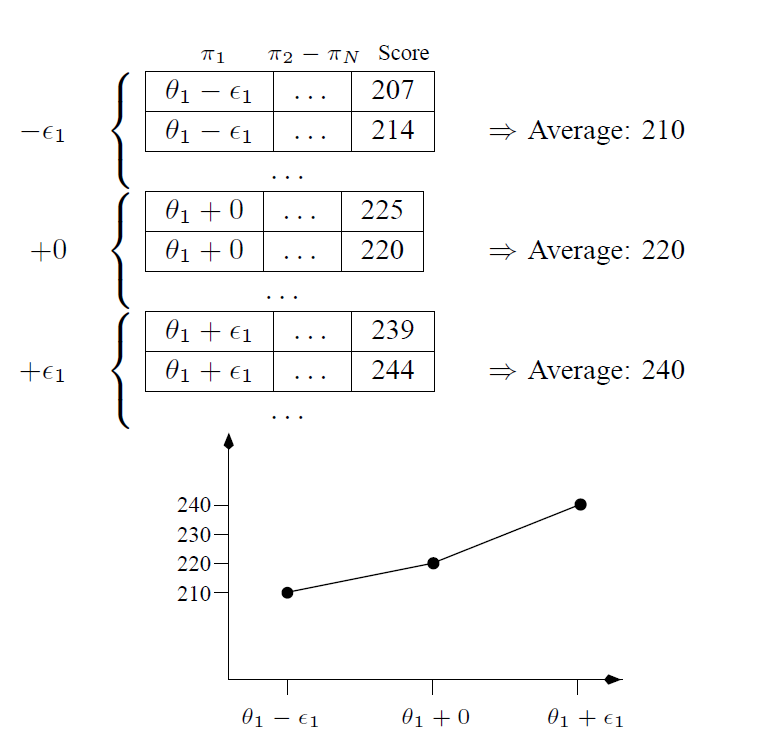
\includegraphics[width=0.5\textwidth]{figures/l9-training-diff.png}\\
  \caption{The policy updates}\label{fig:training-diff}
  \end{centering}
\end{figure}




\subsection{AlphaGo}

AlphaGo and its successor AlphaGo Zero are the most advanced
computer Go players, and the first to beat the best professional
players. We will concentrate on AlphaGo. AlphaGo Zero has an
additional benefit that it does not have any prior information about
the game (mainly in the form of games between human experts).

The training has roughly three phases. The first phase learns from
from human games (played by experts). Those games are used to derive
a network SL (Supervised Learning) to predict next move of the
human, and a Rollout which is a simple but very fast prediction (3
orders faster than SL).

During phase two an RL network is trained. It is initialized with SL
weights, and is optimized on self-play against itself.

In phase three, a value network is trained to predict the winner of
the game (trained on the RL network self-play games). (See
Figure~\ref{fig:AlphaGo-arch}.)


\begin{figure}
  % Requires \usepackage{graphicx}
  \begin{centering}
  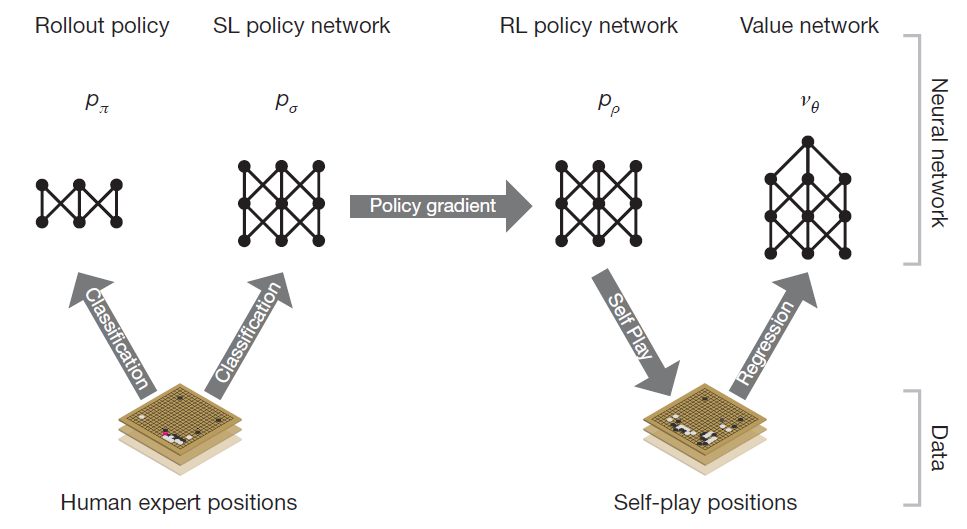
\includegraphics[width=\textwidth]{figures/AlphaGo-arch.PNG}\\
  \caption{The AlphaGo training process}\label{fig:AlphaGo-arch}
  \end{centering}
\end{figure}

\paragraph{Phase 1}\ \\
The SL network is trained to predict the human moves. It is a deep
network (13 layers), and the goal is to output
$p(\action|\state;\sigma)$ where $\sigma$ are the parameters of the
network. The parameters are update using a gradient step,
\[
\Delta \sigma \propto \frac{\partial \log
p(\action|\state;\sigma)}{\partial \sigma}
\]
Overall, this network increased the prediction accuracy (compared to
previous computer programs) from 44\% to 55\%. We should note that
the increase in accuracy translated to a much more significant
improvement in the performance.

In addition to SL, another very fast classifier Rollout was build.
It uses a linear function approximation and predicts using a
soft-max. The accuracy is only 24\% but it is much faster ($2\mu s$
compared to $3ms$,  a factor of $1500$).

\paragraph{Phase 2}\ \\
We learn an RL network that outputs $p(\action|\state;\rho)$ where
$\rho$ are the parameters of the network. The network structure is
identical to that of SL, and the RL is initialized to the weights of
SL, i.e., $\sigma$.

The RL is trained using self-play. Rather then playing against the
most recent network, the opponent is selected at random between the
recent RL configurations. This is done to avoid overfitting. The
rewards of the game are given only at the end (win or lose).

The training is done using SGD with policy gradient
\[
\Delta \rho \propto \frac{\partial \log
p(\action|\state;\rho)}{\partial \rho}
\]

The learned RL network outperformed SL (wins 80\%) of the games.
However, SL is better in predicting expert human behavior.

\paragraph{Phase 3}\ \\
We learn a value function $V(\state;\theta)$. The goal is to predict
the probability that RL will win, and it is trained on the self-play
data of RL. It uses a SGD update
\[
\Delta \theta \propto \frac{\partial V(\state;\theta)}{\partial
\theta}
\]

When the training was done on complete games, there was a serious
problem of over-fitting. (The training error was $0.19$ while the
test error was $0.37$). For this reason, the training is limited to
only one position per game. The error rate is about $0.22$.

The system uses a Monte-Carlo Search Trees (MCST) to evaluate the
positions. The tree is used to perform a lookahead. It uses the
Rollout policy to generate trajectory from the given position. The
prediction is an average of the value network prediction
$V(\state;\theta)$ and the outcome of the Rollout policy. To see a
run of the Monte-Carlo Search Tree see
Figure~\ref{fig:AlphaGo-MCST}.


\begin{figure}
  % Requires \usepackage{graphicx}
  \begin{centering}
  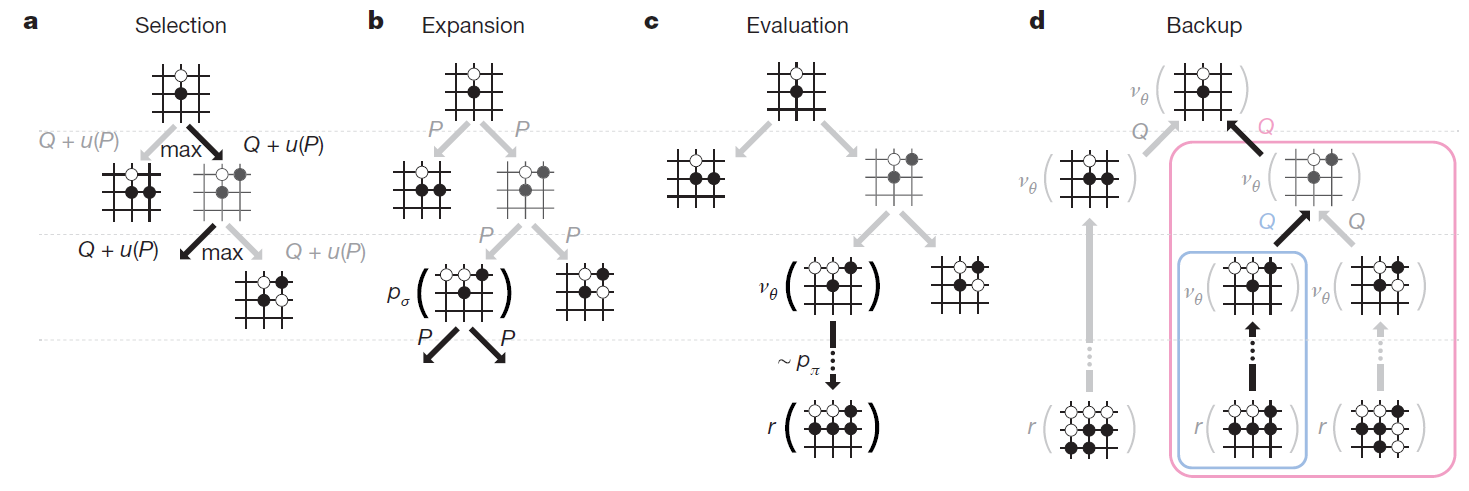
\includegraphics[width=\textwidth]{figures/AlphaGo-MCST.PNG}\\
  \caption{AlphaGo use of Monte-Carlo trees}\label{fig:AlphaGo-MCST}
  \end{centering}
\end{figure}

\section{Bibliography Remarks}

The training of Aibo for RoboSoccer is by \cite{KohlS04}.

The work on AlphaGo is by \cite{SilverHMGSDSAPL16}.

Part of the outline borrows from David Silver class notes and the
the book of Sutton and Barto \cite{SuttonB98}.
